\chapter{Požadavky a návrh prostředí pro NVF a VFN}

V předešlé kapitole byla vysvětlena základní problematika, která souvisí s virtualizací síťových funkcí, cloud computingem a softwarově definovanými sítěmi. Zároveň byla popsána referenční architektura frameworku pro virtualizaci síťových funkcí a popsána existující řešení vhodná pro jednotlivé části architektury.

Tato kapitola bude již věnována konkrétnímu návrhu platformy pro testování NFV a VNF. Nejprve jsou zde popsány jednotlivé požadavky související s návrhem platformy pro NFV a následně jsou popsány požadavky i na jednotlivé VNF. Na základě těchto požadavků je poté navrhuta a popsána výsledná architektura.

\section{Požadavky a výběr platformy pro NFV Infrastrukturu}

V předchozí kapitole bylo řečeno, že existuje několik možností, jakými může být NFV infrastruktura vytvořena. Z tohoto důvodu musí být definované specifické požadavky, které by měla splňovat NFV infrastruktura pro účely této práce. Podle nich následně může být zvolena specifická technologie. Na základě již uvedených informací o NFV a cílů této práce byli identifikovány následující požadavky:

\begin{itemize}
\item Otevřenost řešení - Vzhledem k tomu, že NFV je založeno na myšlence přechodu z proprietárních hardwarových boxů k standarním sofwarově definovaným funkcím, tak je rozumné využít opensource technologie i pro NFV Infrastrukturu. 
\item Možnost automatizace a vytváření templatů - Jedním z cílů práce je VNF řešení, které by mohlo sloužit jako blueprint pro ostatní uživatelé. Proto musí být zvolené technologie, které mají podporu vytváření templatů. Těmi může být následně automaticky vytvořino celé či alespoň část řešení pro VNF. Zárověň však jejich tvorba musí být dostatečně flexibilní a jednoduchá, aby ji zvládli i uživatelé.
\item Podpora SDN - Dalším důležitým požadavkem je podpora softwarově definovaných sítí. Jak již bylo řečeno, tak přestože NFV a SDN jsou odlišené technologie, tak se velice dobře doplňují. Z tohoto důvodu by zvolená platforma pro NFV Infrastrukturu mělo podporovat i SDN. Díky tomu následně může být využíván service chainig pro jednotlivá VNF. 
\end{itemize}

Na základě těchto požadavků je v následující tabulce je uvedeno srovnání cloudových platforem z předchozí kapitoli.

\newcommand{\mc}[2]{\multicolumn{#1}{c}{#2}}
\definecolor{Gray}{gray}{0.85}
\definecolor{LightCyan}{rgb}{0.88,1,1}
\newcolumntype{a}{>{\columncolor{Gray}}c}
\newcolumntype{b}{>{\columncolor{white}}c}
\begin{table} [h] \label{tab:vmware_openstack}
\begin{center}
\begin{tabular}{l | a | b | a | b}
\hline
\rowcolor{LightCyan}
\mc{1}{}  & \mc{1}{VMware vCloud Suite} & \mc{1}{OpenStack} \\
\hline
Typ & opensource & proprietaci/licence  \\ 
\hline
Podpora SDN & ANO (VMware NSX) & ANO (OpenContrail)  \\ 
\hline
Service Chaning & ANO & ANO  \\ 
\hline
Tvorba templatů pro orchestraci & Tvorba v GUI &  Tvorba v YAML formátu  \\ 
\hline
\end{tabular}
\caption[Srovnání VMware vCloud Suite a OpenStacku]{Srovnání VMware vCloud Suite a OpenStacku na požadovaných parameterech}
\end{center}
\end{table}

Ná základě těchto informací bylo rozhodnuto, že pro NFV infrastrukturu bude využita cloudová platforma OpenStack.


\section{Požadavky a výběr řešení pro VNF}

Dále je potřeba rozhodnout, který software bude použit pro implementaci jednotlivých VNF. Proto byly opět definované požadavky, které by potencionální software měl splňovat. Tyto požadavky jsou: 

\begin{itemize}
\item Dostupnost - Pro to, aby bylo vůbec možné uvažované řešení použít, tak je nutné, aby bylo dostupné pro testování. Dostupnost může být ve formě opensource či určité formy trial licence. 
\item Kompatibilita s platformou x86 - Dalším požadavkem musí být kompatibilita s paltformou x86. Je tedy nutné, aby mohlo být využito klasických serverů pro řešení. 
\item Úspěšné spuštění na virtualizační platformě - Pro účely této práce musí být ověřeno, že dané řešení je schopné běžet na daném hypervizoru, který bude použit s OpenStackem. Tedy s hypevizorem KVM.
\item Integrace s OpenStackem - V případě LbaaS je požadované, aby vybraný software měl určitou formu integrace s prostředím OpenStacku. Je to z důvodu lepší automatizace VNF.
\end{itemize}

Následující tabulka nabízí přehled toho, zda daný software splňuje určené požadavky.


\definecolor{Gray}{gray}{0.85}
\definecolor{LightCyan}{rgb}{0.88,1,1}
\newcolumntype{a}{>{\columncolor{Gray}}c}
\newcolumntype{b}{>{\columncolor{white}}c}
\begin{table} [h] \label{tab:vmware_openstack}
\begin{center}
\begin{tabular}{l | a | b | a | b}
\hline
\rowcolor{LightCyan}
\mc{1}{LbaaS}  & \mc{1}{HAproxy} & \mc{1}{AVI networks} \\
\hline
Dostupnost & ANO - opensource & ANO - Trial licence  \\ 
\hline
Integrace s OpenStackem & ANO (default) & ANO - plugin  \\ 
\hline
Úspěšné spuštění & ANO & ANO  \\ 
\hline
Kompatibilita x86 & ANO & ANO  \\ 
\hline
\end{tabular}
\caption[Přehled softwaru pro LbaaS]{Přehled softwaru pro LbaaS}
\end{center}
\end{table} 


\definecolor{Gray}{gray}{0.85}
\definecolor{LightCyan}{rgb}{0.88,1,1}
\newcolumntype{a}{>{\columncolor{Gray}}c}
\newcolumntype{b}{>{\columncolor{white}}c}
\begin{table} [h] \label{tab:vmware_openstack}
\begin{center}
\begin{tabular}{l | a | b | a | b}
\hline
\rowcolor{LightCyan}
\mc{1}{FwaaS}  & \mc{1}{Fortigate VM} & \mc{1}{Juniper vSRX} & \mc{1}{Cisco ASAv} & \mc{1}{PfSense} \\
\hline
Dostupnost & ANO - Trial & ANO - Trial & NE - Licence  & ANO - opensource    \\ 
\hline
Úspěšné spuštění & ANO & NE  & NE & ANO   \\ 
\hline
Kompatibilita x86 & ANO & ANO & ANO & ANO  \\ 
\hline
\end{tabular}
\caption[Přehled softwaru pro FwaaS]{Přehled softwaru pro FwaaS}
\end{center}
\end{table} 

Z výše uvedených informací vyplívá, že pro implementaci LbaaS bude použita HAproxy a platforma, kterou poskytuje firma AVI networks. V případě softwaru pro FwaaS je zrejmé, že bude využit PfSense a Fortigate VM v 15 denní trial verzi. Cisco ASAv nebylo možné testovat kvůli licenčním poplatkům a Juniper vSRX se bohužel nepodařilo zprovoznit v KVM hypervizoru na testovací infrastruktuře.

\section{Výsledná architektura použitého frameworku}

V předchozích částech byly vybrány technologie, které jsou použity v návrhu pro NFV framework. Na obrázku č. \ref{fig:VNF_overview} je znázornění celého framework s vyobrazením všech použitých částí.

\begin{figure}[h]
\begin{centering}
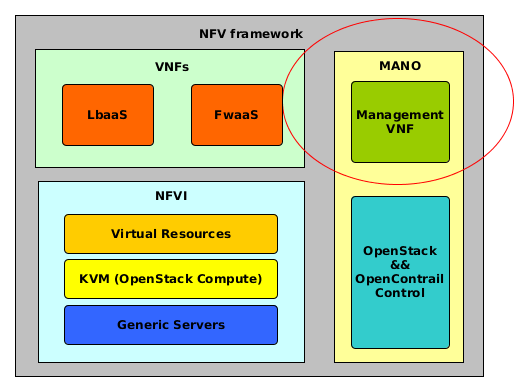
\includegraphics[scale=0.61]{images/VNF_overview}
\par\end{centering}
\caption{Architektura NFV řešení\label{fig:VNF_overview}}
\end{figure}

Z obrázku je patrné, že celou NFV Infrastrukturu tvoří OpenStack s SDN řešením OpenContrail. Ty zasahují i managementu a orchestrace na nejnižší úrovni. Jako hypervizor byl použit KVM. Jako VNF služby budou poskytovány Load Balancer a Firewall. Poslední částí, kterou se bude zabývat zbytek práce je management jednotlivých VNF.

Pro fyzické vytvoření frameworku bylo využito 4 serverů. Jeden slouží jako Control node, na kterém jsou řídící služby OpenStacku a OpenContrailu společně s jejich dashboardy. Zbylé 3 servery jsou použity jako Compute nody. Na nich nainstalovaný hypervisor společně s compute rolemi OpenStacku. Dále je na nich i OpenContrail vRouter. Pomocí něho je vytvořený tzv. Overlay network, který používají vytvořené instance.


\begin{figure}[h]
\begin{centering}
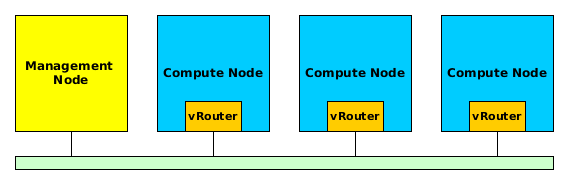
\includegraphics[scale=0.61]{images/fyzicka_topologie}
\par\end{centering}
\caption{Architektura NFV řešení\label{fig:fyzicka_topologie}}
\end{figure}
